\section{Burndown Chart}\label{sec:burndown}
The burndown chart seen below shows the current status of project in the middle of sprint 2 and also the estimated progress of the project in its entirety. The blue line represents the actual progress and the red line the estimated progress. We estimated our initial velocity to be around 35 story points per sprint. The reason for that being that we would need time to get used to the work environment and new tools. We finished all the stories in the first sprint so we estimated a considerable increase in velocity given that the adjustment period was over. We estimated 65 story points per sprint for the next five sprints and then 145 story points per sprint for the last two sprints since the team's capacity was much higher then as the team members had no other courses to worry about. 

\begin{figure}[H]
	\centering

    \centerline{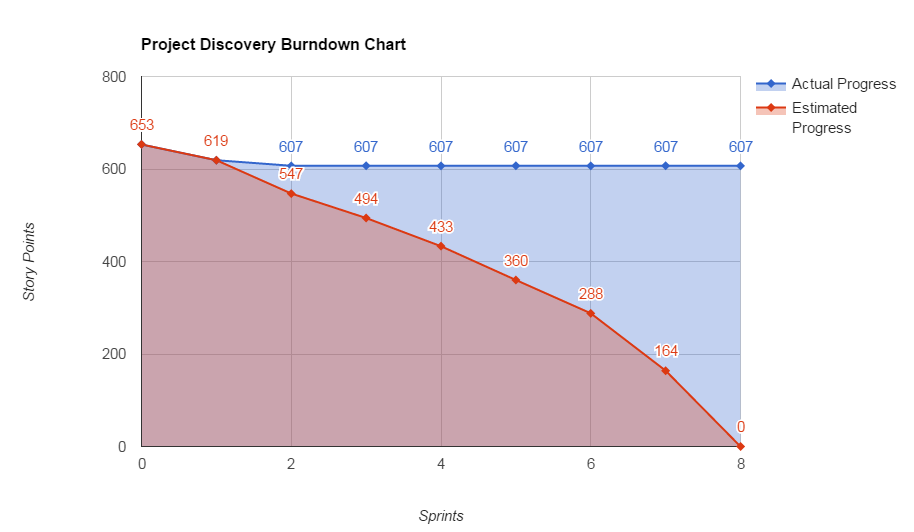
\includegraphics[scale=0.6]{bdchart.png}}
    \caption{\label{fig:PD}Burndown chart in sprint 2}
\end{figure}